\section{Dexterity Network}
\seclabel{dexnet}

The Dexterity Network (Dex-Net) 1.0 dataset is a growing set that currently includes over 10,000 prior 3D object models annotated with 2.5 million parallel-jaw grasps.
Dex-Net 1.0 contains 13,252 models from the following sources: 8,987 from the SHREC 2014 challenge dataset~\cite{li2015comparison}, 2,539 from ModelNet40~\cite{wu20153d}, 1,371 from 3DNet~\cite{wohlkinger20123dnet}, 129 from the KIT object database~\cite{kasper2012kit}, 120 from BigBIRD~\cite{singh2014bigbird}, 80 from the Yale-CMU-Berkeley dataset~\cite{calli2015benchmarking}, and 26 from the Amazon Picking Challenge scans.

\subsection{Data Cleaning}
Each object in Dex-Net is specified as a 3D mesh.
We preprocess each mesh by removing unreferenced vertices, computing a reference frame with Principal Component Analysis (PCA) on the mesh vertices, setting the mesh center of mass $\bz$ to the center of the mesh bounding box, and rescaling the synthetic meshes to fit the smallest dimension of the bounding box within $w = 0.1m$, which is approximately the maximal opening width of a PR2 gripper.
We also convert each mesh to an SDF $f$ using SDFGen~\cite{sdfgen}.

\subsection{Grasp Sampling}
\seclabel{grasp-sampling}
Each 3D object $\mO_i$ in Dex-Net is labelled with up to 250 parallel-jaw grasps and their $P_F$.
We generate $N_g$ grasps for each object using a modification of the 2D algorithm presented in Smith et al.~\cite{smith1999computing} to concentrate samples on grasps that are antipodal~\cite{mahler2015gp}.
Let $w$ be the maximal opening of the gripper, $\hat{\gamma}$ be a sampled friction coefficient, and $\mS$ be the set of points on the object surface for an SDF $f$ as described in \secref{grasp-param}.
To sample a single grasp, we first generate a contact point $\bc_1$ by sampling uniformly from $\mS$.% using rejection sampling.
Next we sample a direction $\bv \in \bS^2$ uniformly at random from the friction cone and compute $\bc_2 = \bc_1 + (w / 2 - t_2^*) \bv$ and $\bx = 0.5 (\bc_1 + \bc_2)$, where $t_2^*$ is defined in \secref{contact}.
This yields a grasp $\bg_{i,k} = (\bx, \bv)$.
We add $\bg_{i,k}$ to the candidate set if the contacts are antipodal~\cite{mahler2015gp}, or $\bv^T \bn_1 \leq \cos(\arctan(\hat{\gamma}))$ and $\bv^T \bn_2 \leq \cos(\arctan(\hat{\gamma}))$.

We evaluate $P_F(\bg)$ using Monte-Carlo integration~\cite{kehoe2012toward} by sampling the object pose, gripper pose, and friction random variables $N_s$ times and recording $S_{i,k}$, the number of samples for which grasp $\bg_{i,k}$ was in force closure.
The full dataset of $N_o$ 3D objects and $N_g$ grasps per object is $\mD = \{ (S_{i, k}, \mY_{i, k}) \big| i = \{1, ..., N_o\}, k = \{1, ..., N_g\} \}$ where $\mY_{i,k} = (\bg_{i, k}, \mO_i) \in \mM$ is a grasp-object pair in Dex-Net.


%We generate a set of grasps for each object in the network using the method of \secref{candidates} and evaluate the probability of force closure for each grasp using brute-force Monte Carlo integration as a benchmark~\cite{kehoe2012toward}.
%As the number of models is quite large, we distribute the grasp labelling for each object across virtual machines in Google Compute Engine and aggregate the results at the end.

\subsection{Grasp Differential Heightmap Features}
\seclabel{grasp-similarity}
To measure grasp similarity, we embed each grasp $\bg$ on object $\mO$ in Dex-Net in a feature space based on 2D projections of the local surface orientation at the contacts, inspired by grasp heightmaps~\cite{herzog2014learning, kappler2015leveraging}.
Let $d_h \in \mathbb{Z}$ be a number of pixels for the projection, let $\mP = \{-d_h, ..., d_h\}$ be row / column pixel indices, let $\delta \in \mathbb{R}$ be the pixel resolution in meters, and let $r \in \mathbb{R}$ be a minimum projection distance.
%Furthermore, let $\bc_i, i = 1, 2$ be a contact point for grasp $\bg$ and let $\bt_1, \bt_2$ be two orthogonal unit vectors to the grasp approach direction $\bv$.
The heightmap at contact $\bc_i$, $\bh_{i}: \mP \times \mP \rightarrow \bR$, maps discrete locations along the tangent plane to the grasp axis $\bv$ specified by $\bt_1, \bt_2$ to the distance to the surface along $\bv$.
To compute the value at pixel $u,v \in \mP$, we compute the location of the pixel on the plane $\bp_i(u,v) = \bc_i + \delta u \bt_1 + \delta v \bt_2$ and assign
\begin{align*}
	\bh_i(u,v) = \minimum{t \geq -r} t \text{ such that } f\left( \bp_i(u,v) + (-1)^{i} t \bv \right) = 0
\end{align*}
\noindent where $f$ is the SDF of object $\mO$. 
We make $\bh_i$ rotation-invariant by orienting its axes to align with the eigenvectors of the weighted covariance matrix of the 3D surface points that generate the heightmap as described in~\cite{salti2014shot}.
\figref{local-feature-model} illustrates local surface patches extracted by this procedure.
Since force closure depends on object surface normals at contacts~\cite{pokorny2013c}, we finally take the $x$- and $y$-image gradients of $\bh_i$ to form differential heightmaps $\bd_{i,x}$ and $\bd_{i,y}$.
The full feature vector for each grasp-object pair  in Dex-Net is $\eta(\bg, \mO) = (\bd_{1,x}, \bd_{1,y}, \bd_{2,x}, \bd_{2,y})$.

\begin{figure}[t!]
\centering
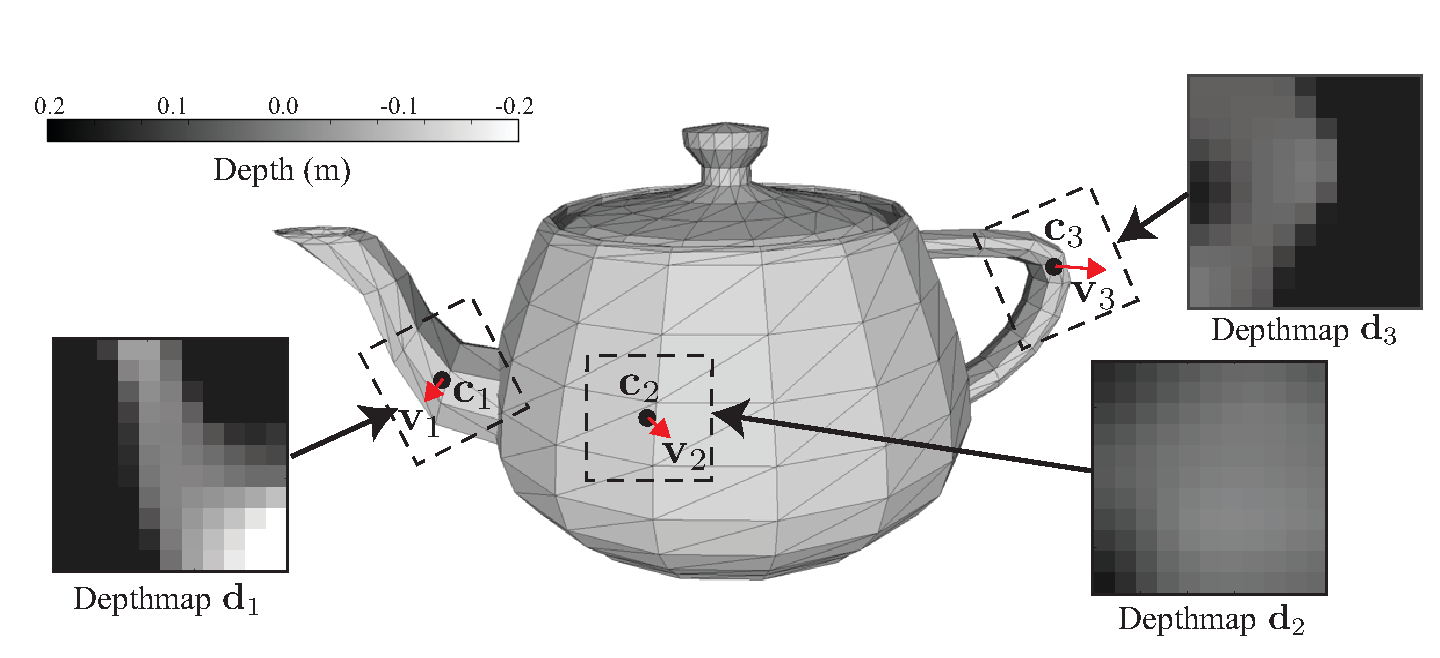
\includegraphics[scale=0.30]{figures/illustrations/local_feature_model.eps}
\caption{Illustration of three local surface heightmaps extracted on a teapot. Each heightmap is ``rendered" along the grasp axis $\bv_i$ at contact $\bc_i$ and oriented by the directions of maximum variation in the heightmap.  We use gradients of the heightmaps for similiarity between grasps in Dex-Net.}
\figlabel{local-feature-model}
\vspace*{-15pt}
\end{figure}

\section{Deep Learning for Object Similarity}
\seclabel{object-similarity}
We use Multi-View Convolutional Neural Networks (MV-CNNs)~\cite{aubry2015understanding, su2015multi} to efficiently index prior 3D object and grasp data from Dex-Net by embedding each object in a vector space where distance represents object similarity, as shown in \figref{global-feature-model}.
We first render every object on a white background in a total of $N_c = 50$ virtual camera views oriented toward the object center and discretized on a viewing sphere along angle increments $\delta_{\theta} = \frac{4 \pi}{N_c}$ and $\delta_{\phi} = \frac{2 \pi}{N_c}$ and radii $r = R, 2R$, where $R$ is the maximum dimension of the object bounding box.
Then we train a CNN with the architecture of AlexNet~\cite{krizhevsky2012imagenet} to predict the 3D object class label for the rendered images on a training set of models. 
We initialize the weights of the network with the weights learned on ImageNet by Krizhevsky et al.~\cite{krizhevsky2012imagenet} and optimize using Stochastic Gradient Descent (SGD). 
Next, we pass each of the $N_c$ views of each object through the optimized CNN and max-pool the output of the fc7 layer, the highest layer of the network before the class label prediction. 
Finally, we use Principal Component Analysis (PCA) to reduce the max-pooled output from 4,096 dimensions to 100 dimensions.
This yields the representation $\psi(\mO) \in \mathbb{R}^{100}$ for each object.

Given the MV-CNN object representation, we measure the dissimilarity between two objects $\mO_i$ and $\mO_j$ by the Euclidean distance $\| \psi(\mO_i) - \psi(\mO_j) \|_2$.
For efficient lookups of similar objects, Dex-Net contains a KD-Tree nearest neighbor query structure with the feature vectors of all prior objects.
In our implementation, we trained the MV-CNN using the Caffe library~\cite{jia2014caffe} on rendered images from a training set of approximately $6,000$ 3D models from the SHREC 2014 dataset ~\cite{li2015comparison} for 500,000 iterations of SGD.
%The final PCA step captured approximately 85\% of the variance of the vectors.
%The image classification training step had a test accuracy of 76\%.
To validate the implementation, we tested on the SHREC 2014 challenge dataset and achieved a 1-NN accuracy of 86.7\%, compared to 86.8\% achieved by the winner of SHREC 2014~\cite{li2015comparison}.

\begin{figure}[t!]
\centering
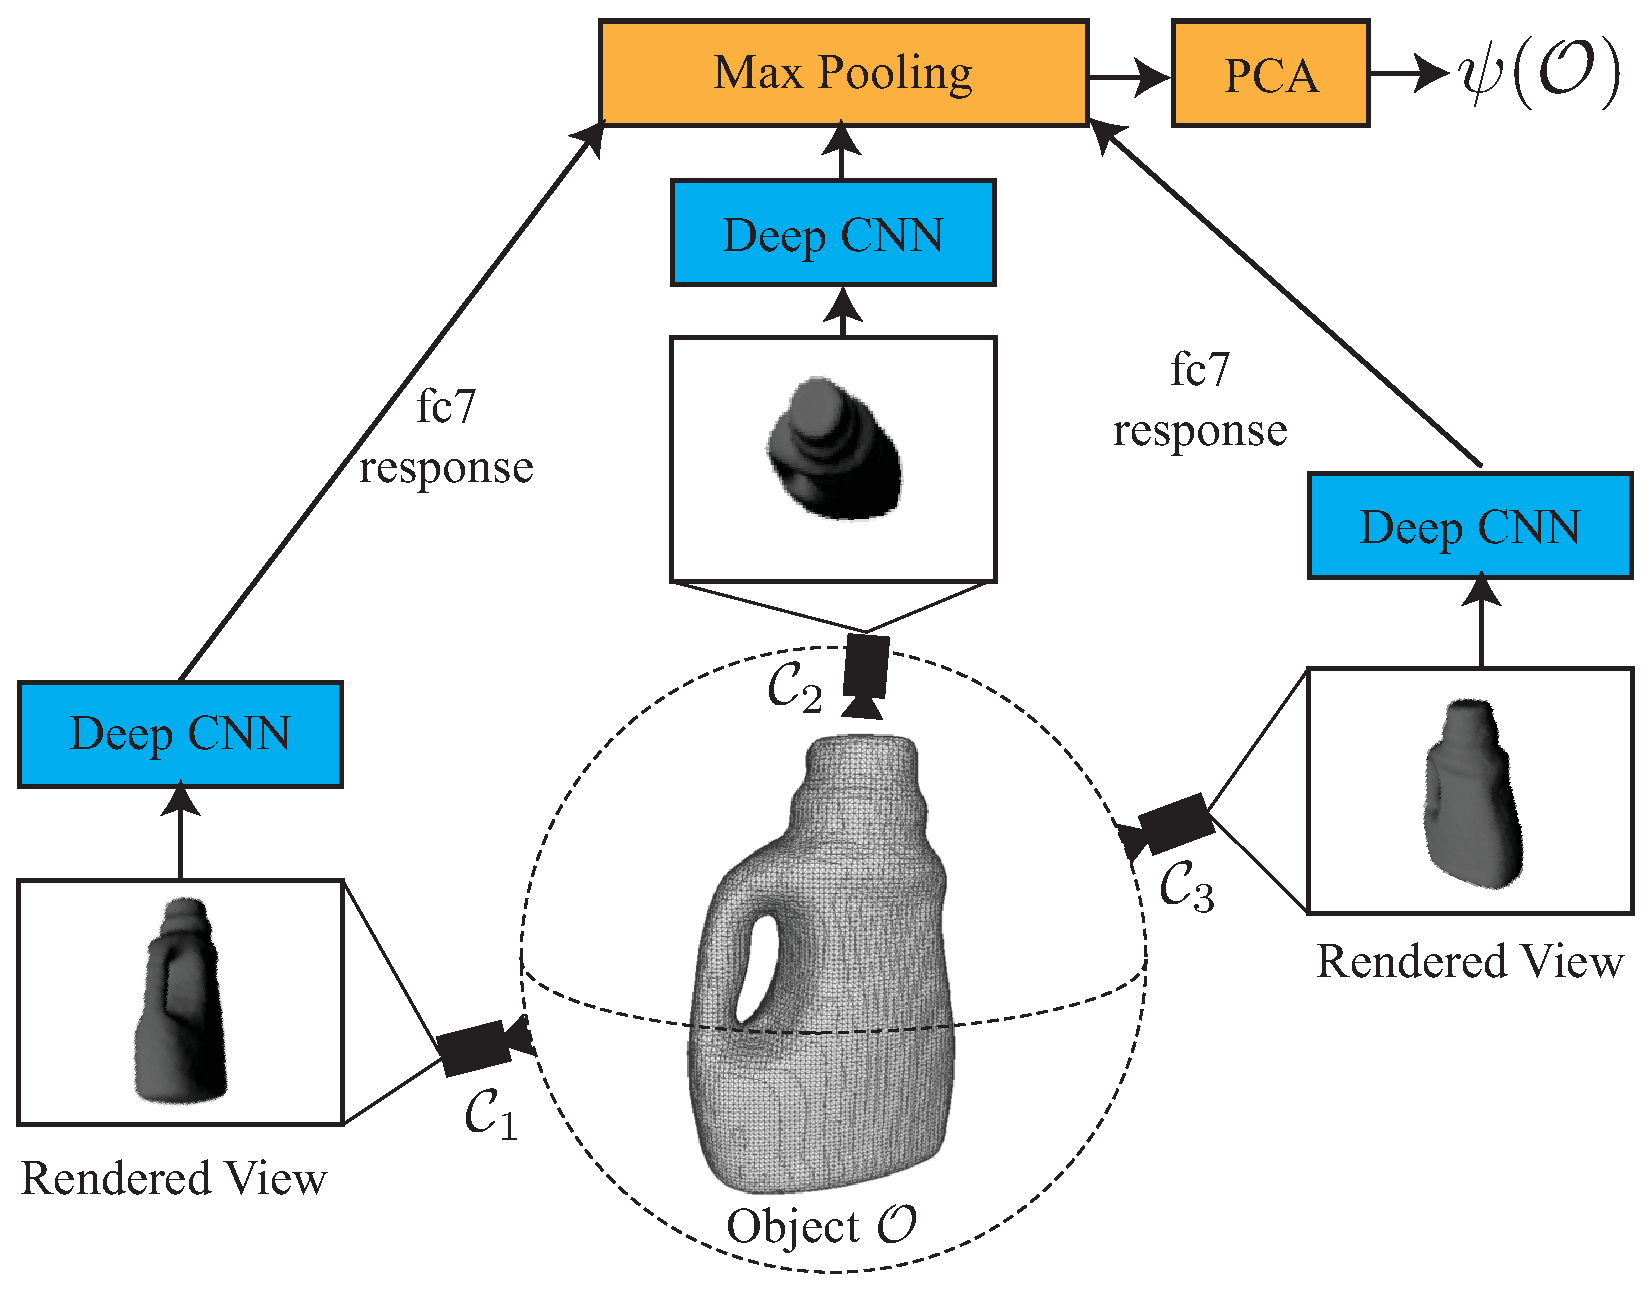
\includegraphics[scale=0.275]{figures/illustrations/cnn_model.eps}
\caption{Illustration of our Multi-View Convolutional Neural Network (MV-CNN) deep learning method for embedding 3D object models in a Euclidean vector space to compu global shape similiarty. We pass a set of 50 virtually rendered camera viewpoints discretized around a sphere through a deep Convolutional Neural Network (CNN) with the AlexNet~\cite{krizhevsky2012imagenet} architecture. Finally, we take the maximum fc7 response across each of the 50 views for each dimension and run PCA to reduce dimensionality.}
\figlabel{global-feature-model}
\vspace*{-15pt}
\end{figure}

